\documentclass[11pt,a4paper]{article}
\usepackage[utf8]{inputenc}
\usepackage[margin=0.75in]{geometry}
\usepackage{hyperref}
\usepackage{booktabs}
\usepackage{xcolor}
\usepackage{listings}
\usepackage{tikz}
\usetikzlibrary{shapes.multipart,arrows.meta,positioning,fit}
\usepackage{titlesec}
\usepackage{microtype}

\titleformat{\section}{\large\bfseries\color{blue!70!black}}{\thesection}{1em}{}[\titlerule]
\titleformat{\subsection}{\normalsize\bfseries\color{black!85}}{\thesubsection}{1em}{}

\hypersetup{
    colorlinks=true,
    linkcolor=blue!70!black,
    urlcolor=blue!70!black,
    citecolor=blue!70!black
}

\lstset{
    basicstyle=\ttfamily\footnotesize,
    breaklines=true,
    frame=single,
    rulecolor=\color{gray!40},
    backgroundcolor=\color{gray!5},
    keywordstyle=\color{blue!80!black}\bfseries,
    commentstyle=\color{green!50!black}\itshape,
    stringstyle=\color{red!70!black},
    numbers=none
}

\begin{document}

\begin{center}
    {\Large \textbf{ASTANA IT UNIVERSITY}}\\[0.2em]
    {\large Department of Software Engineering \textbar{} ShP-2216 Software Design Patterns}\\[0.4em]
    {\LARGE \textbf{Assignment 06: Advanced In-Memory File System}}\\[0.2em]
    {\large \textbf{Visitor Pattern \& Double Dispatch Architecture}}\\[0.5em]
    \textbf{Student:} Dias \quad \textbar{} \quad \textbf{Weight:} 15\% of RK2 \quad \textbar{} \quad \textbf{Java 17 \textbar{} Maven \textbar{} JUnit 5}\\[0.3em]
    \textbf{GitHub Repository:} \url{https://github.com/Dias-AITU/sdp-assignment-06-visitor}
\end{center}

\vspace{-0.5em}
\hrule
\vspace{0.8em}

% -----------------------------------------------------------------------------
\section{Purpose and Architectural Design Choices}
% -----------------------------------------------------------------------------
The objective of this assignment is to design an in-memory hierarchical file system that decouples structural object representation from arbitrary domain operations using the \textbf{Visitor Behavioral Pattern} and \textbf{Composite Structural Pattern}.

\subsection{Double Dispatch Mechanics and Elimination of Type Inspection}
Traditional object hierarchies often succumb to fragile \texttt{instanceof} cascades, reflection, or type-based branching when new features are added. This solution strictly utilizes \textbf{Double Dispatch}:
\begin{enumerate}\itemsep 0pt
    \item \textbf{First Dispatch (Element Selection):} The client invokes \texttt{element.accept(visitor)}. Runtime polymorphic dispatch dynamically routes the call to the concrete class (\texttt{FileNode} or \texttt{DirectoryNode}).
    \item \textbf{Second Dispatch (Operation Selection):} Inside the concrete element, it invokes \texttt{visitor.visit(this)}. The compiler binds the overloaded visit method based on the exact compile-time type of \texttt{this}, executing either \texttt{visit(FileNode)} or \texttt{visit(DirectoryNode)}.
\end{enumerate}
This pattern guarantees that behavioral selection is performed entirely through dynamic polymorphism with \textbf{zero runtime type checks}.

\subsection{Tree Integrity and Invariant Enforcement (R6)}
The file system preserves structural consistency across all mutations through synchronous assertions in constructors and the composite's \texttt{DirectoryNode.addChild()} method:
\begin{itemize}\itemsep 0pt
    \item \textbf{Non-Negative File Size:} Enforced in \texttt{FileNode(name, size)} via \texttt{InvalidFileSizeException}.
    \item \textbf{Duplicate Sibling Rejection:} \texttt{DirectoryNode} maintains children in a \texttt{LinkedHashMap<String, FileSystemElement>}. If an element with the same name already exists in the target directory, a \texttt{DuplicateNameException} is thrown.
    \item \textbf{Single-Parent Ownership:} Elements verify that \texttt{getParent() == null} before attachment. Attempting to add an element already attached elsewhere throws \texttt{MultipleParentException}.
    \item \textbf{Cycle Prevention:} When adding a child directory, the method iterates upward along the parent pointers of \texttt{this}. If any ancestor equals the incoming child, a \texttt{CycleDetectedException} is thrown.
\end{itemize}

% -----------------------------------------------------------------------------
\section{UML Class Diagram}
% -----------------------------------------------------------------------------
The diagram below illustrates the relationship between the composite element hierarchy and the visitor subsystem:

\begin{center}
\resizebox{0.95\textwidth}{!}{%
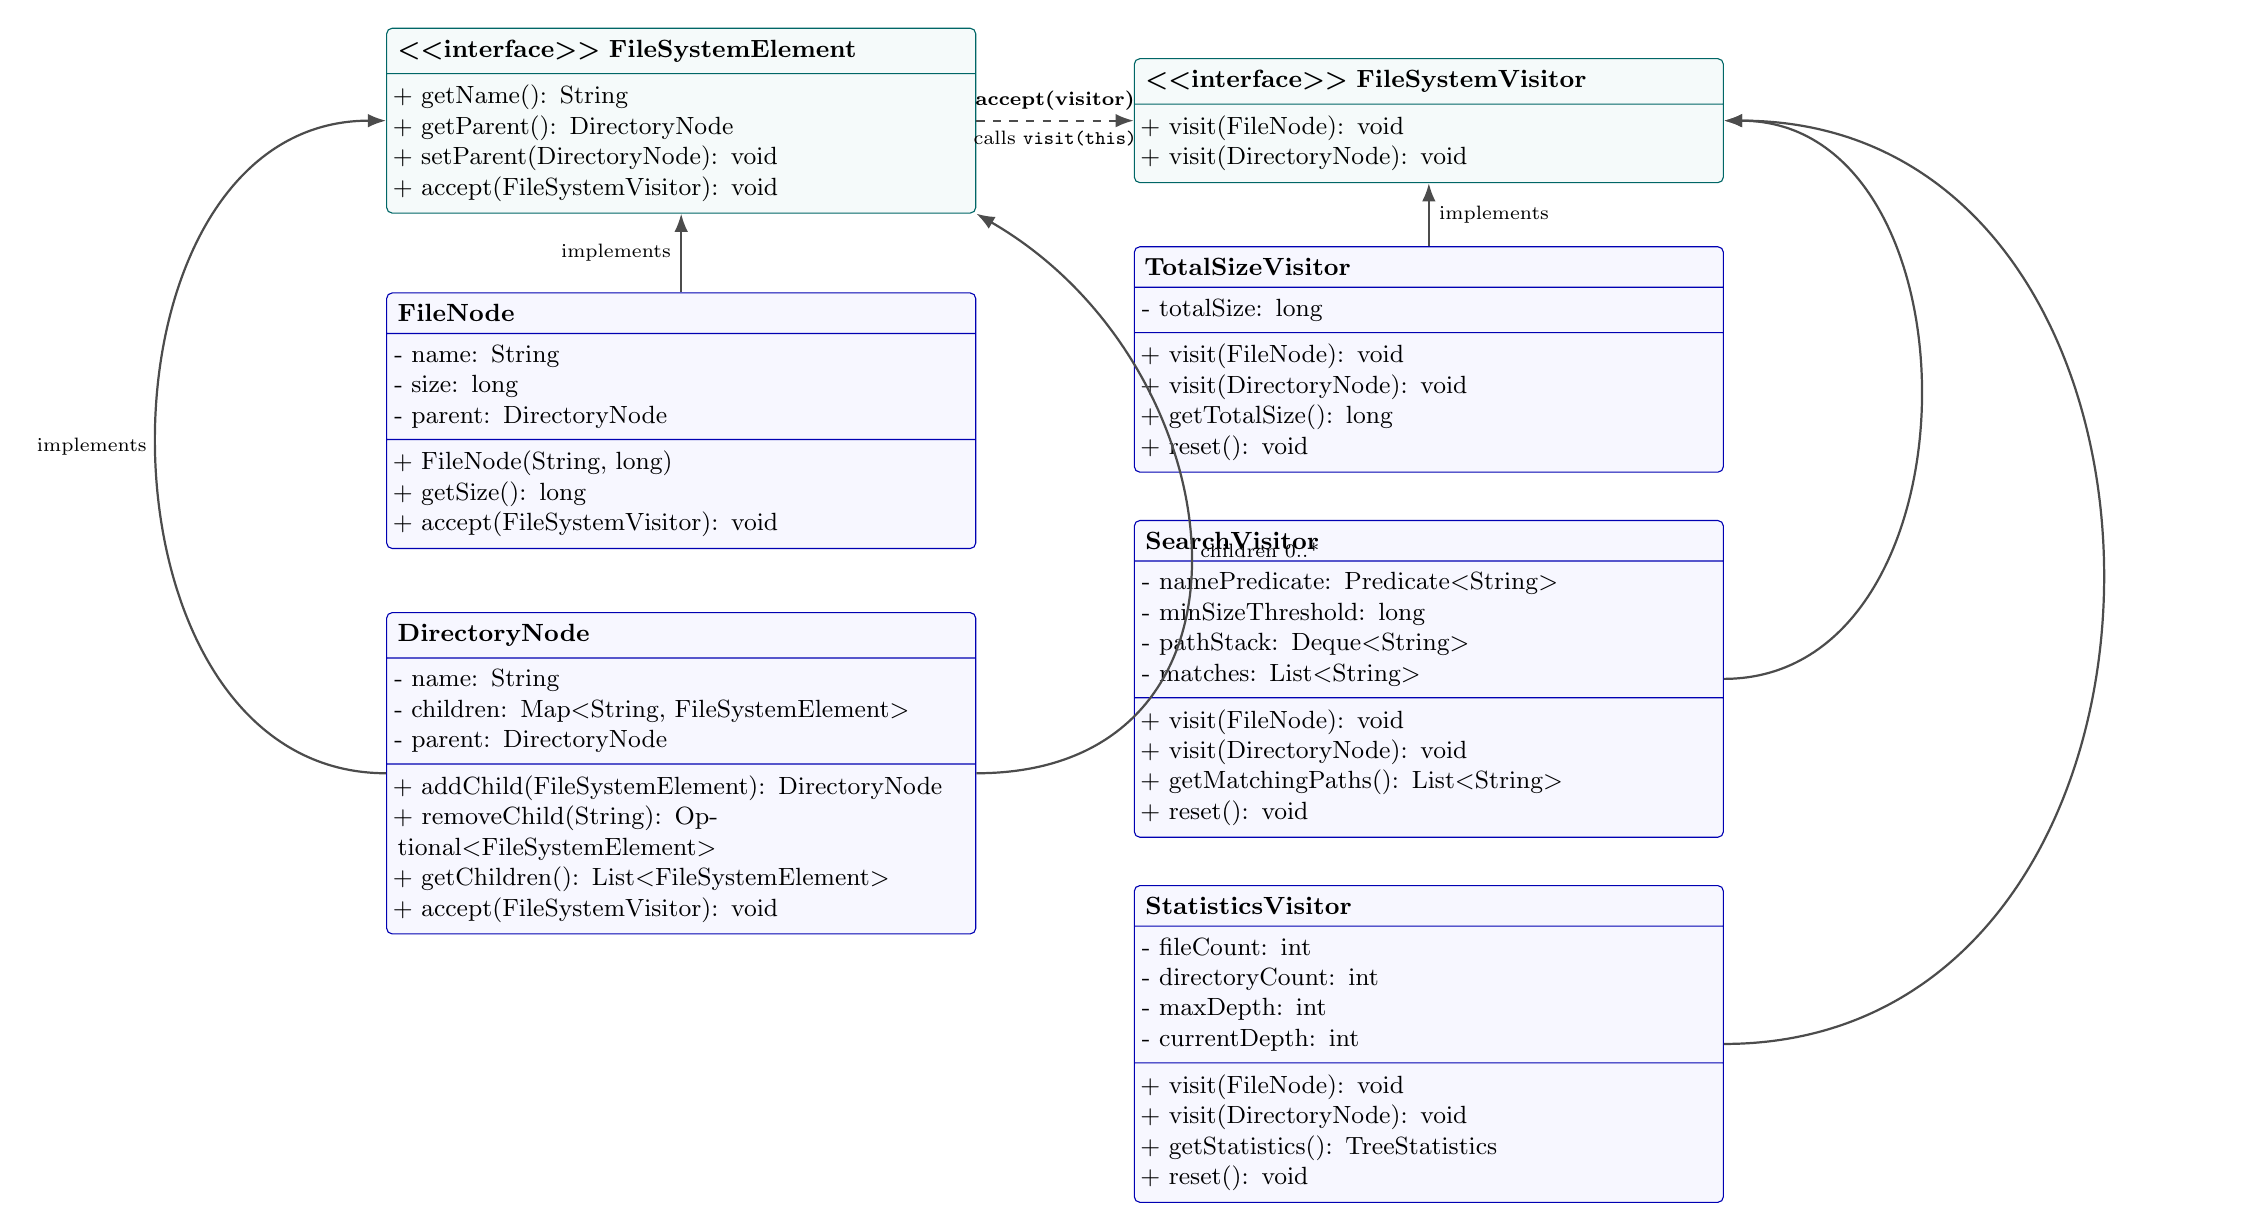
\begin{tikzpicture}[
    classbox/.style={
        rectangle split,
        rectangle split parts=3,
        draw=blue!70!black,
        rounded corners=2pt,
        fill=blue!3,
        text width=7.2cm,
        font=\small,
        inner sep=4pt
    },
    interfacebox/.style={
        rectangle split,
        rectangle split parts=2,
        draw=teal!80!black,
        rounded corners=2pt,
        fill=teal!4,
        text width=7.2cm,
        font=\small,
        inner sep=4pt
    },
    line/.style={-Latex, thick, draw=black!70},
    dashline/.style={-Latex, dashed, thick, draw=black!70}
]

% Left Column: Element Hierarchy
\node[interfacebox] (element) {
    \textbf{\textless\textless interface\textgreater\textgreater{} FileSystemElement}
    \nodepart{second}
    + getName(): String\\
    + getParent(): DirectoryNode\\
    + setParent(DirectoryNode): void\\
    + accept(FileSystemVisitor): void
};

\node[classbox, below=1.0cm of element] (filenode) {
    \textbf{FileNode}
    \nodepart{second}
    - name: String\\
    - size: long\\
    - parent: DirectoryNode
    \nodepart{third}
    + FileNode(String, long)\\
    + getSize(): long\\
    + accept(FileSystemVisitor): void
};

\node[classbox, below=0.8cm of filenode] (dirnode) {
    \textbf{DirectoryNode}
    \nodepart{second}
    - name: String\\
    - children: Map\textless String, FileSystemElement\textgreater\\
    - parent: DirectoryNode
    \nodepart{third}
    + addChild(FileSystemElement): DirectoryNode\\
    + removeChild(String): Optional\textless FileSystemElement\textgreater\\
    + getChildren(): List\textless FileSystemElement\textgreater\\
    + accept(FileSystemVisitor): void
};

% Right Column: Visitor Hierarchy
\node[interfacebox, right=2.0cm of element] (visitor) {
    \textbf{\textless\textless interface\textgreater\textgreater{} FileSystemVisitor}
    \nodepart{second}
    + visit(FileNode): void\\
    + visit(DirectoryNode): void
};

\node[classbox, below=0.8cm of visitor] (sizevis) {
    \textbf{TotalSizeVisitor}
    \nodepart{second}
    - totalSize: long
    \nodepart{third}
    + visit(FileNode): void\\
    + visit(DirectoryNode): void\\
    + getTotalSize(): long\\
    + reset(): void
};

\node[classbox, below=0.6cm of sizevis] (searchvis) {
    \textbf{SearchVisitor}
    \nodepart{second}
    - namePredicate: Predicate\textless String\textgreater\\
    - minSizeThreshold: long\\
    - pathStack: Deque\textless String\textgreater\\
    - matches: List\textless String\textgreater
    \nodepart{third}
    + visit(FileNode): void\\
    + visit(DirectoryNode): void\\
    + getMatchingPaths(): List\textless String\textgreater\\
    + reset(): void
};

\node[classbox, below=0.6cm of searchvis] (statsvis) {
    \textbf{StatisticsVisitor}
    \nodepart{second}
    - fileCount: int\\
    - directoryCount: int\\
    - maxDepth: int\\
    - currentDepth: int
    \nodepart{third}
    + visit(FileNode): void\\
    + visit(DirectoryNode): void\\
    + getStatistics(): TreeStatistics\\
    + reset(): void
};

% Relationships
\draw[line] (filenode.north) -- node[left,font=\scriptsize]{implements} (element.south);
\draw[line] (dirnode.west) to[out=180,in=180,looseness=1.2] node[left,font=\scriptsize]{implements} (element.west);
\draw[line] (dirnode.east) to[out=0,in=-30,looseness=1.4] node[right,font=\scriptsize]{children 0..*} (element.south east);

\draw[line] (sizevis.north) -- node[right,font=\scriptsize]{implements} (visitor.south);
\draw[line] (searchvis.east) to[out=0,in=0,looseness=1.2] (visitor.east);
\draw[line] (statsvis.east) to[out=0,in=0,looseness=1.4] (visitor.east);

\draw[dashline] (element.east) -- node[above,font=\scriptsize]{\textbf{accept(visitor)}} node[below,font=\scriptsize]{calls \texttt{visit(this)}} (visitor.west);

\end{tikzpicture}%
}
\end{center}

\newpage

% -----------------------------------------------------------------------------
\section{Clean Code Justifications}
% -----------------------------------------------------------------------------
The code adheres strictly to established Clean Code principles:

\begin{enumerate}\itemsep 4pt
    \item \textbf{Meaningful Naming (\texttt{SearchVisitor.buildRootRelativePath()}):}\\
    The method name explicitly communicates intent (constructing a `/`-separated path relative to the traversal root) without requiring inline explanatory comments.
    \item \textbf{Single Responsibility Principle (\texttt{DirectoryNode} vs. \texttt{TotalSizeVisitor}):}\\
    \texttt{DirectoryNode} is solely responsible for maintaining child element relationships and enforcing tree integrity invariants, while calculation algorithms (size, search, statistics) are isolated inside independent visitor classes.
    \item \textbf{Small, Focused Methods (\texttt{FileNode.accept()} and \texttt{DirectoryNode.accept()}):}\\
    The dispatch methods contain a single statement delegating to \texttt{visitor.visit(this)}, keeping cyclomatic complexity at exactly 1 and maximizing testability.
    \item \textbf{Encapsulation of Internal State (\texttt{DirectoryNode.getChildren()}):}\\
    The internal mutable child map is completely shielded from external modification by returning \texttt{Collections.unmodifiableList(new ArrayList<>(children.values()))}.
    \item \textbf{Elimination of Type-Checking Chains (\texttt{FileSystemElement.accept()}):}\\
    No \texttt{instanceof}, reflection, or conditional branching exists to differentiate between files and directories; method routing is handled entirely by double dispatch polymorphism.
\end{enumerate}

% -----------------------------------------------------------------------------
\section{Architectural and Extension Trade-Offs}
% -----------------------------------------------------------------------------

\subsection{Traversal Ownership: Visitor-Owned vs. Element-Owned (R7)}
We selected \textbf{Visitor-Driven Traversal}. In this architecture, composite elements expose their unmodifiable children, and each visitor dictates how and when to traverse them.
\begin{itemize}\itemsep 1pt
    \item \textbf{Advantage 1 (Context Tracking):} Operations such as \texttt{SearchVisitor} and \texttt{StatisticsVisitor} require contextual state (a path stack for root-relative paths and a current depth counter). The visitor pushes state before visiting child nodes and pops state upon return. If traversal were embedded in \texttt{DirectoryNode}, this context would have to be passed awkwardly through element method arguments.
    \item \textbf{Advantage 2 (Traversal Control):} Specific visitors can prune branches (e.g., skip hidden or permission-restricted folders) without polluting the composite element's structure.
\end{itemize}

\subsection{Extension Boundary Trade-Offs (The Visitor Dilemma)}
The Visitor pattern introduces an explicit architectural trade-off:
\begin{itemize}\itemsep 1pt
    \item \textbf{Adding Operations (Extremely Easy):} Adding a new operation, such as \texttt{StatisticsVisitor} (R8) or a hypothetical \texttt{ChecksumVisitor}, is achieved by creating a new class implementing \texttt{FileSystemVisitor}. Zero lines of code in \texttt{FileNode}, \texttt{DirectoryNode}, or existing visitors are modified. The Open-Closed Principle is strictly upheld.
    \item \textbf{Adding Element Types (Hard):} If a new element type is introduced (e.g., \texttt{SymlinkNode}), the \texttt{FileSystemVisitor} interface must add \texttt{visit(SymlinkNode)}, which immediately breaks and requires updates across all existing visitor implementations (\texttt{TotalSizeVisitor}, \texttt{SearchVisitor}, and \texttt{StatisticsVisitor}).
\end{itemize}

% -----------------------------------------------------------------------------
\section{Verification Suite \& Execution Output}
% -----------------------------------------------------------------------------

\subsection{Automated JUnit 5 Test Suite Results}
All 8 mandatory verification targets executed cleanly using \texttt{mvn test} with zero failures:
\begin{center}
\footnotesize
\begin{tabular}{lp{6.8cm}p{5.2cm}c}
\toprule
\textbf{Check} & \textbf{Test Method Name} & \textbf{Verification Target} & \textbf{Result} \\
\midrule
T1 & \texttt{testT1\_DoubleDispatchReaches...} & Pure double dispatch routing & \textbf{PASSED} \\
T2 & \texttt{testT2\_SizeAccumulationAcross...} & Multi-level subtree byte size & \textbf{PASSED} \\
T3 & \texttt{testT3\_SearchCombinesName...} & Dual-filter search constraints & \textbf{PASSED} \\
T4 & \texttt{testT4\_SearchProducesDeterministic...} & Lexicographically sorted `/` paths & \textbf{PASSED} \\
T5 & \texttt{testT5\_StatisticsCorrectForNesting...} & File/dir count \& max tree depth & \textbf{PASSED} \\
T6 & \texttt{testT6\_EmptyStructuresAndNoMatch...} & Empty directories \& search misses & \textbf{PASSED} \\
T7 & \texttt{testT7\_RepeatExecutionsDoNotLeak...} & State isolation \& visitor reuse & \textbf{PASSED} \\
T8 & \texttt{testT8\_InvalidTreeMutationsRejected...} & Tree integrity invariants (R6) & \textbf{PASSED} \\
\bottomrule
\end{tabular}
\end{center}

\subsection{Deterministic Program Output (\texttt{kz.aitu.shp.filesystem.Main})}
\begin{lstlisting}
================================================================================
  OPERATION 1: TotalSizeVisitor (R3)
--------------------------------------------------------------------------------
Total Subtree Byte Size: 141180 bytes (137.87 KB)

--------------------------------------------------------------------------------
  OPERATION 2: SearchVisitor (R4)
--------------------------------------------------------------------------------
Query A: Filename contains '.java' AND size >= 3000 bytes
  [1] src/main/java/Application.java
  [2] src/main/java/OrderService.java
  [3] src/test/java/OrderServiceTest.java

Query B: All files with size >= 5000 bytes
  [1] docs/architecture-spec.json
  [2] docs/system-design.pdf
  [3] target/ecommerce-core-1.0.jar

--------------------------------------------------------------------------------
  OPERATION 3: StatisticsVisitor (R5 & R8)
--------------------------------------------------------------------------------
Hierarchy Statistics Summary:
  * Total Files Visited:       14
  * Total Directories Visited: 10 (including root)
  * Maximum Tree Depth:        4 (root depth = 0)

--------------------------------------------------------------------------------
  TREE INTEGRITY ENFORCEMENT (R6)
--------------------------------------------------------------------------------
1. Duplicate sibling prevention: PASSED -> Caught DuplicateNameException
2. Negative size prevention:     PASSED -> Caught InvalidFileSizeException
3. Cycle prevention:             PASSED -> Caught CycleDetectedException
================================================================================
\end{lstlisting}

\end{document}
